\documentclass[12pt]{article}

% Set page size and margins
\usepackage[letterpaper,top=2cm,bottom=2cm,left=3cm,right=3cm,marginparwidth=1.75cm]{geometry}

% Useful packages
\usepackage{graphicx}
\usepackage{amsmath}

\title{AM 213A HW3}
\author{Joseph Moore}
\date{Winter 2022}

\newenvironment{amatrix}[1]{%
	\begin{array}{@{}*{#1}{c}|c@{}}
	}{%
	\end{array}
}

\begin{document}

\maketitle

\title{\textbf{Part 1}}
 
\paragraph{a)}
	\subparagraph{$\bullet$}
		The first ten singular values are as follows,
		\[\begin{matrix}
		\sigma_1 = 663180.202318 \\
		\sigma_2 = 85706.595735 \\
		\sigma_3 = 62129.025680 \\
		\sigma_4 = 34664.633004 \\
		\sigma_5 = 31861.792296 \\
		\sigma_6 = 21872.721620 \\
		\sigma_7 = 19628.442780 \\
		\sigma_8 = 18434.937653 \\
		\sigma_9 = 13693.815446 \\
		\sigma_{10} = 12815.208252.
		\end{matrix}	
		\]
		The $k^{th}$ singular values are as follows,
		\[\begin{matrix}
		\sigma_{20} = 7528.024652  \\
		\sigma_{40} = 5489.124664  \\
		\sigma_{80} = 3948.779979  \\
		\sigma_{160} = 2668.223578 \\
		\sigma_{320} = 1515.865932 \\
		\sigma_{640} = 821.893126  \\
		\sigma_{1280} = 513.568032 \\
		\sigma_{2560} = 179.115035 \\
		\end{matrix}	
		\]
		The very last singular value is $\sigma_{3355} = 16.724645$

\newpage	
	\subparagraph{$\bullet$}
		The matrix of singular values corresponds to the level of image compression depicted below.\\
	
		$\Sigma_{\sigma_{20}}$ creates the image \\
		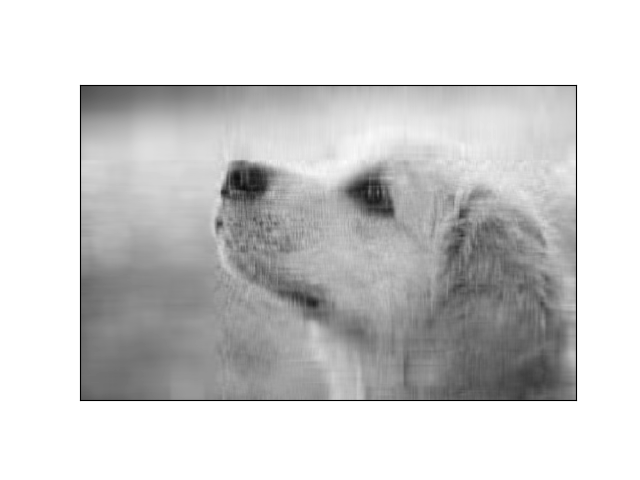
\includegraphics[scale=0.8]{part1/prob_a/Figure_1} \\
		$\Sigma_{\sigma_{40}}$ creates the image \\
		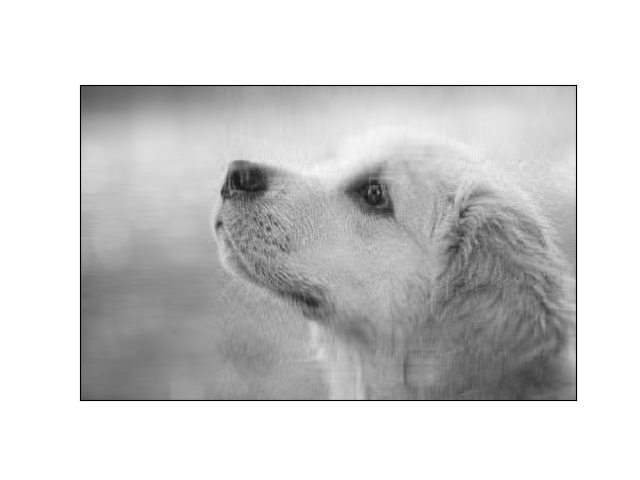
\includegraphics[scale=0.8]{part1/prob_a/Figure_2} \\
\newpage
		$\Sigma_{\sigma_{80}}$ creates the image \\
		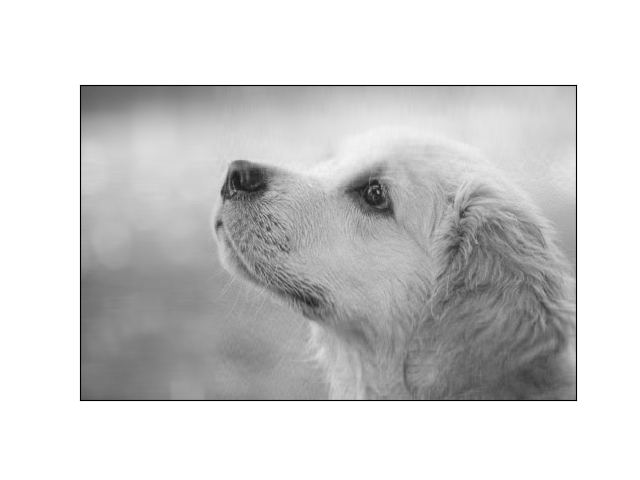
\includegraphics[scale=0.8]{part1/prob_a/Figure_3} \\
		$\Sigma_{\sigma_{160}}$ creates the image \\
		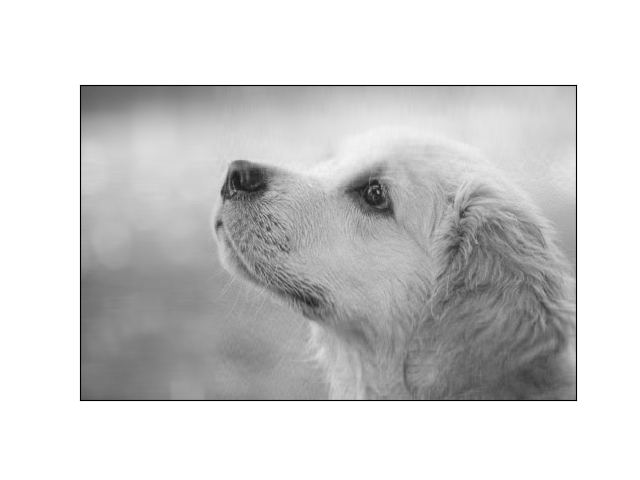
\includegraphics[scale=0.8]{part1/prob_a/Figure_4} \\
\newpage
		$\Sigma_{\sigma_{320}}$ creates the image \\
		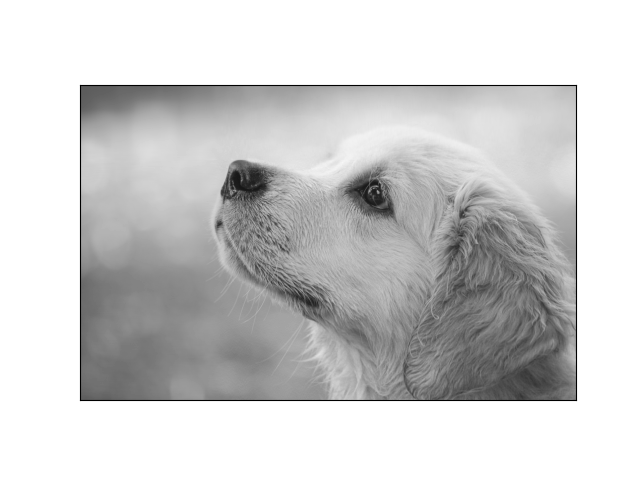
\includegraphics[scale=0.8]{part1/prob_a/Figure_5} \\
		$\Sigma_{\sigma_{640}}$ creates the image \\
		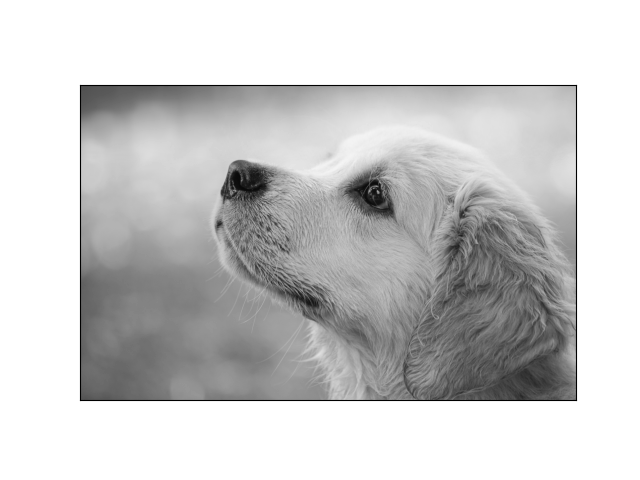
\includegraphics[scale=0.8]{part1/prob_a/Figure_6} \\
\newpage
		$\Sigma_{\sigma_{1280}}$ creates the image \\
		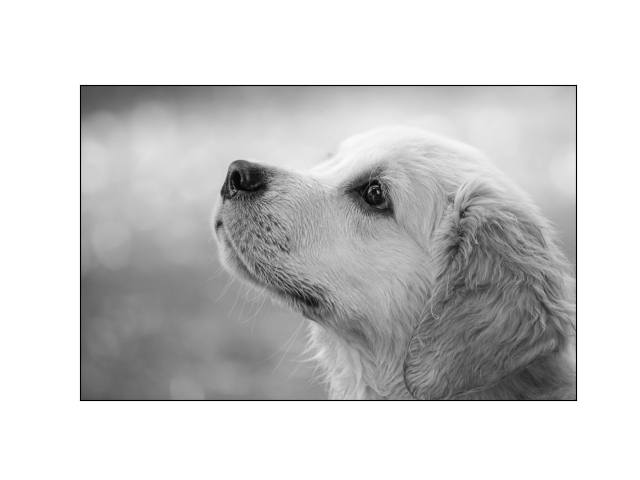
\includegraphics[scale=0.8]{part1/prob_a/Figure_7} \\
		$\Sigma_{\sigma_{2560}}$ creates the image \\
		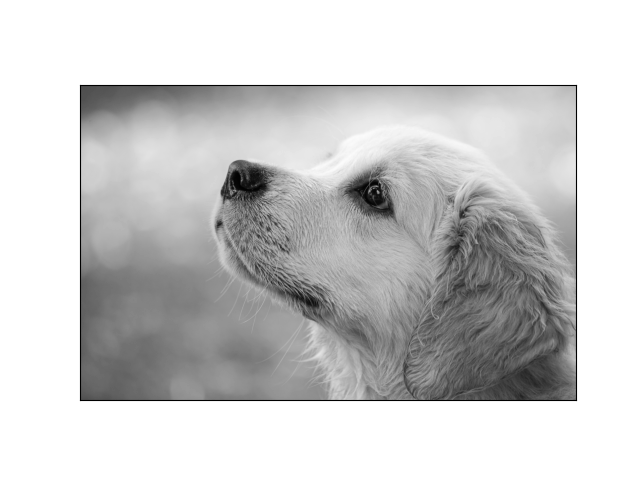
\includegraphics[scale=0.8]{part1/prob_a/Figure_8} \\
\newpage		
		$\Sigma_{\sigma_{3355}}$ is the all the singular values and thus is the original image \\
		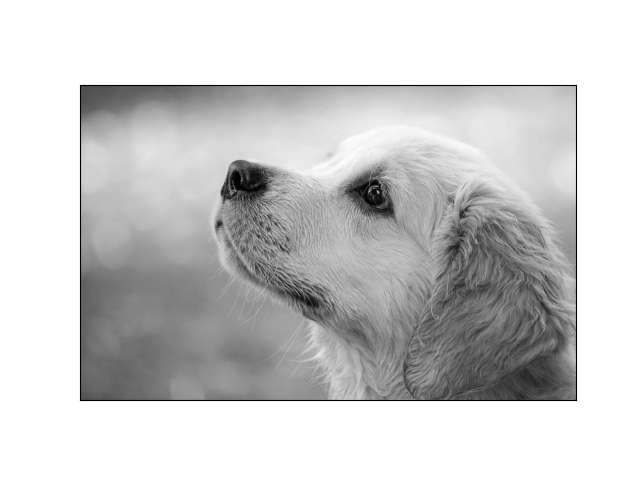
\includegraphics[scale=0.8]{part1/prob_a/Figure_9} \\

	\subparagraph{$\bullet$}	
		\[
		E_{20} = \frac{||A - A_{\sigma_{20}}||_F}{mn} = 0.003543
		\]\[
		E_{40} = \frac{||A - A_{\sigma_{40}}||_F}{mn} = 0.003166
		\]\[
		E_{80} = \frac{||A - A_{\sigma_{80}}||_F}{mn} = 0.002703
		\]\[
		E_{160} = \frac{||A - A_{\sigma_{160}}||_F}{mn} = 0.002156
		\]\[
		E_{320} = \frac{||A - A_{\sigma_{320}}||_F}{mn} = 0.001604
		\]\[
		E_{640} = \frac{||A - A_{\sigma_{640}}||_F}{mn} = 0.001173
		\]\[
		E_{1280} = \frac{||A - A_{\sigma_{1280}}||_F}{mn} = 0.000711
		\]\[
		E_{2560} = \frac{||A - A_{\sigma_{2560}}||_F}{mn} = 0.000187
		\]
		
		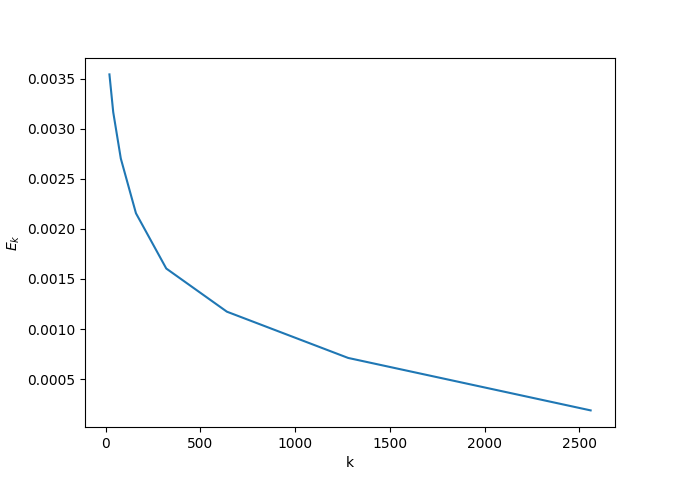
\includegraphics{part1/prob_a/Figure_10}
		
		As the number of singular values increases the image becomes closer to the original. The error falls like $\frac{1}{k}$ and appears to asymptotically approach zero. This tells us that we can get most of the information we need from the first few singular values. The higher we up k the less information is added to our image. At $k = 1280$ the error is below $10^{-3}$. However, from the graph we can tell that the error drops below $10^{-3}$ closer to $k = 1000$. With far less than half the total number of singular values we have a very small error.
	
\paragraph{b.1)}
	\subparagraph{$\bullet$}
		Both the Gauss-Jacobi and the Gauss-Seidel use an iterative method to solve $Ax = b$ for $x$. The Gauss-Jacobi simply splits up $A$ into its diagonal and remaining elements like $A = D + R$ and then follows $x^{k+1} = D^{-1}(b - Rx^k)$ until $x$ converges to a result. Gauss-Jacobi converges when $\rho(D^{-1}R) < 1$. Gauss-Jacobi further splits $R$ into upper and lower triangular matrices so that $A = L + D + U$. Gauss-Seidel follows $x^{k+1} = D^{-1}(b - Lx^{k+1} - Ux^{k})$ and converges for any symmetric, positive definite matrix. Gauss-Seidel converges faster than Gauss-Jacobi when they both converge. 
		
	\subparagraph{$\bullet$}	

	
\newpage	
\title{\textbf{Part 2}}

\paragraph{1.}

	
\paragraph{7.}
	\subparagraph{a)}

	
	\subparagraph{b)}
	
	
\end{document}